\documentclass[]{article}
\usepackage{lmodern}
\usepackage{amssymb,amsmath}
\usepackage{ifxetex,ifluatex}
\usepackage{fixltx2e} % provides \textsubscript
\ifnum 0\ifxetex 1\fi\ifluatex 1\fi=0 % if pdftex
  \usepackage[T1]{fontenc}
  \usepackage[utf8]{inputenc}
\else % if luatex or xelatex
  \ifxetex
    \usepackage{mathspec}
  \else
    \usepackage{fontspec}
  \fi
  \defaultfontfeatures{Ligatures=TeX,Scale=MatchLowercase}
\fi
% use upquote if available, for straight quotes in verbatim environments
\IfFileExists{upquote.sty}{\usepackage{upquote}}{}
% use microtype if available
\IfFileExists{microtype.sty}{%
\usepackage{microtype}
\UseMicrotypeSet[protrusion]{basicmath} % disable protrusion for tt fonts
}{}
\usepackage[margin=1in]{geometry}
\usepackage{hyperref}
\hypersetup{unicode=true,
            pdftitle={SEA 2018 report},
            pdfborder={0 0 0},
            breaklinks=true}
\urlstyle{same}  % don't use monospace font for urls
\usepackage{graphicx,grffile}
\makeatletter
\def\maxwidth{\ifdim\Gin@nat@width>\linewidth\linewidth\else\Gin@nat@width\fi}
\def\maxheight{\ifdim\Gin@nat@height>\textheight\textheight\else\Gin@nat@height\fi}
\makeatother
% Scale images if necessary, so that they will not overflow the page
% margins by default, and it is still possible to overwrite the defaults
% using explicit options in \includegraphics[width, height, ...]{}
\setkeys{Gin}{width=\maxwidth,height=\maxheight,keepaspectratio}
\IfFileExists{parskip.sty}{%
\usepackage{parskip}
}{% else
\setlength{\parindent}{0pt}
\setlength{\parskip}{6pt plus 2pt minus 1pt}
}
\setlength{\emergencystretch}{3em}  % prevent overfull lines
\providecommand{\tightlist}{%
  \setlength{\itemsep}{0pt}\setlength{\parskip}{0pt}}
\setcounter{secnumdepth}{5}
% Redefines (sub)paragraphs to behave more like sections
\ifx\paragraph\undefined\else
\let\oldparagraph\paragraph
\renewcommand{\paragraph}[1]{\oldparagraph{#1}\mbox{}}
\fi
\ifx\subparagraph\undefined\else
\let\oldsubparagraph\subparagraph
\renewcommand{\subparagraph}[1]{\oldsubparagraph{#1}\mbox{}}
\fi

%%% Use protect on footnotes to avoid problems with footnotes in titles
\let\rmarkdownfootnote\footnote%
\def\footnote{\protect\rmarkdownfootnote}

%%% Change title format to be more compact
\usepackage{titling}

% Create subtitle command for use in maketitle
\newcommand{\subtitle}[1]{
  \posttitle{
    \begin{center}\large#1\end{center}
    }
}

\setlength{\droptitle}{-2em}
  \title{SEA 2018 report}
  \pretitle{\vspace{\droptitle}\centering\huge}
  \posttitle{\par}
  \author{}
  \preauthor{}\postauthor{}
  \date{}
  \predate{}\postdate{}


\begin{document}
\maketitle

{
\setcounter{tocdepth}{2}
\tableofcontents
}
\section{Experimental setup}\label{experimental-setup}

\subsection{Time measurements}\label{time-measurements}

We run a program \(k\) times with and without the optimization and
recorded the sum construction time of the MS and RUNS vectors. The plots
report (median, with quartile ranges) of the speedup of each optimized
time \(t_i^{\mathtt{opt}}\) relative to the average non-optimized time
in the construction time of the MS vector. In other words\\
\[
d^{(i)} = \frac{\bar{t}_{\mathtt{non\_opt}}}{t^{(i)}_{\mathtt{opt}}}
\] with
\(\bar{t}_{\mathtt{non\_opt}} = 1/n \sum t^{(i)}_{\mathtt{non\_opt}}\),
and \(i = 1, \ldots, k\).

The boxplots report the raw times.

\section{WL tests}\label{wl-tests}

\subsection{Input data}\label{input-data}

We perform tests on the Weiner Link optimizations on 4 types of input.

\begin{itemize}
\tightlist
\item
  Index string with repeats, query string random (code:
  \texttt{rep\_dis})
\item
  Index string with repeats, query string similar to index (code:
  \texttt{rep\_sim})
\item
  Index string random, query string random (code: \texttt{rnd\_dis})
\item
  Index string random, query string similar to index (code:
  \texttt{rnd\_sim})
\end{itemize}

Further, we generate all of the above input data for two alphabet sizes:
\(\Sigma_1| = 4\) and \(\Sigma_2| = 20\). For all input types, the index
string is of length 100MB and the query 500KB.

\subsection{Double rank}\label{double-rank}

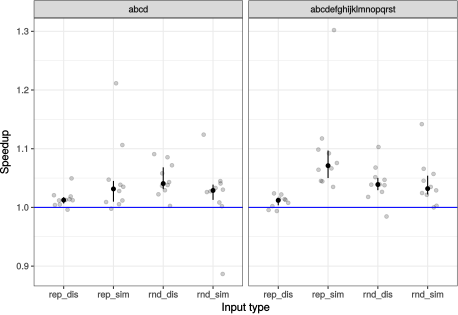
\includegraphics{sea_2018_files/figure-latex/drank_plot_better-1.pdf}
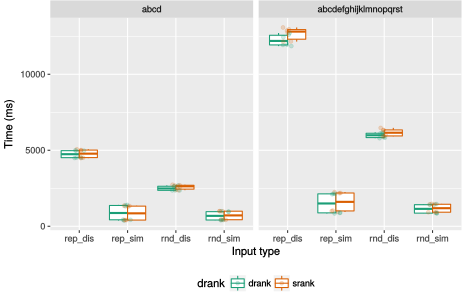
\includegraphics{sea_2018_files/figure-latex/drank_plot_better-2.pdf}

\subsection{Lazy}\label{lazy}

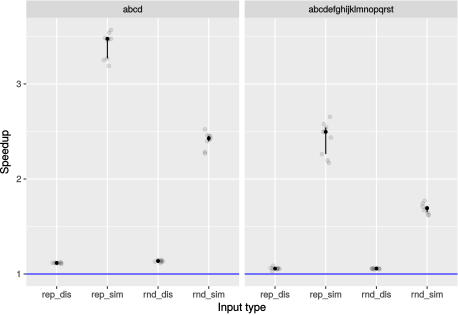
\includegraphics{sea_2018_files/figure-latex/lazy_plot-1.pdf}
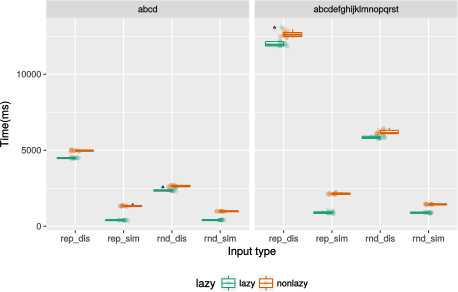
\includegraphics{sea_2018_files/figure-latex/lazy_plot-2.pdf}

\subsection{Rank and fail}\label{rank-and-fail}

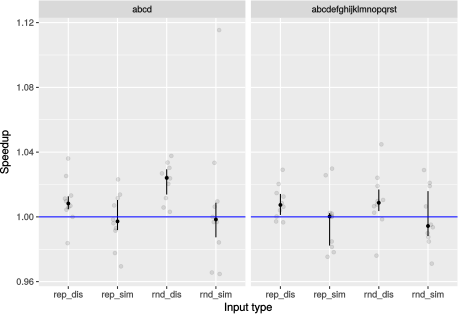
\includegraphics{sea_2018_files/figure-latex/fail_plot-1.pdf}
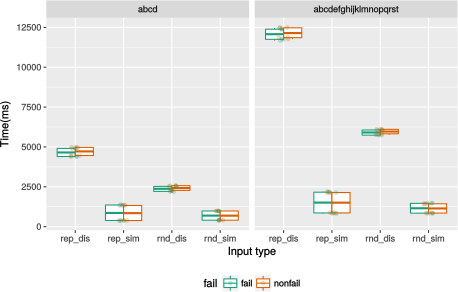
\includegraphics{sea_2018_files/figure-latex/fail_plot-2.pdf}

\subsection{Double rank, Lazy, and Rank and fail versus Single
rank}\label{double-rank-lazy-and-rank-and-fail-versus-single-rank}

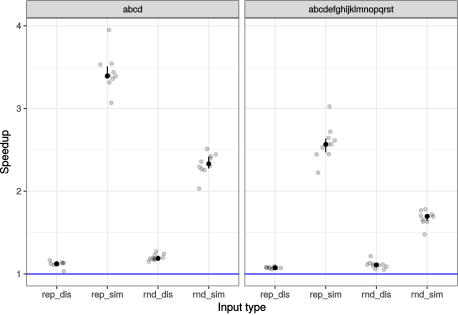
\includegraphics{sea_2018_files/figure-latex/allflags_plot-1.pdf}
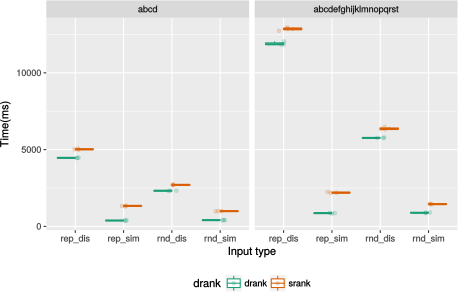
\includegraphics{sea_2018_files/figure-latex/allflags_plot-2.pdf}

\subsection{Maxrep}\label{maxrep}

\subsubsection{Vanilla Maxrep
vs.~non-maxrep}\label{vanilla-maxrep-vs.non-maxrep}

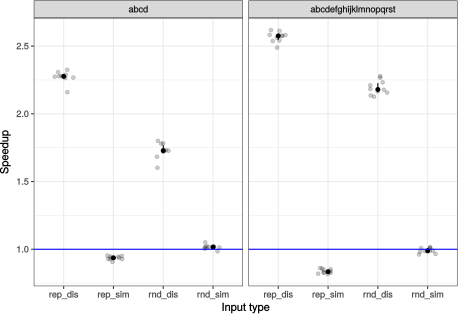
\includegraphics{sea_2018_files/figure-latex/maxrep1_plot-1.pdf}
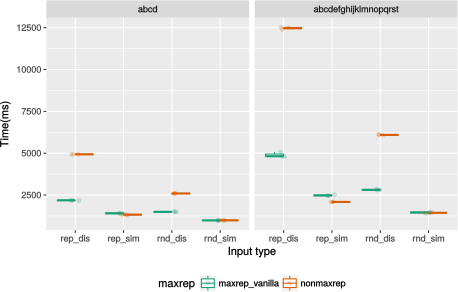
\includegraphics{sea_2018_files/figure-latex/maxrep1_plot-2.pdf}

\subsubsection{Rank and check maxrep versus
non-maxrep}\label{rank-and-check-maxrep-versus-non-maxrep}

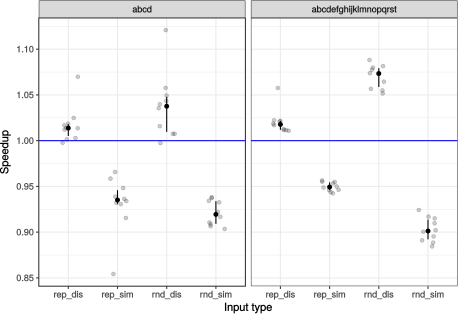
\includegraphics{sea_2018_files/figure-latex/maxrep2_plot-1.pdf}
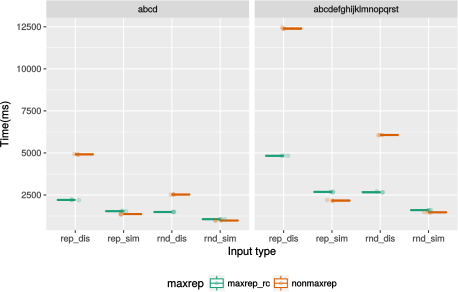
\includegraphics{sea_2018_files/figure-latex/maxrep2_plot-2.pdf}

\subsubsection{Rank and check maxrep versus Vanilla
maxrep}\label{rank-and-check-maxrep-versus-vanilla-maxrep}

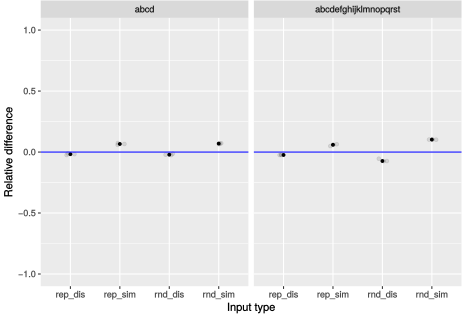
\includegraphics{sea_2018_files/figure-latex/maxrep3_plot-1.pdf}
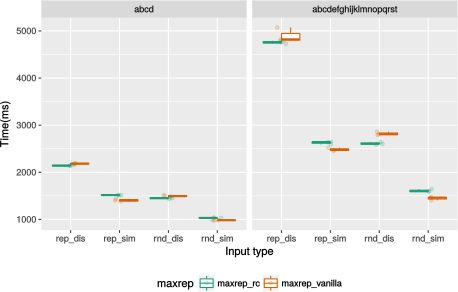
\includegraphics{sea_2018_files/figure-latex/maxrep3_plot-2.pdf}

\section{Optimizations on parent
operations}\label{optimizations-on-parent-operations}

\subsection{Input data}\label{input-data-1}

We generate the index input string with repetitions as follows. We
generate a random seed block \(b\) of length 200. Next, we generate
blocks of the same length \(b_k\) by introducing \(k\) mutations on
\(b\). The index string of length 10MB is
\(b\circ b_k^{(1)} \ldots \circ b_k^{(4999)}\).

The query string is obtained as a concatenation of labels from nodes of
the suffix tree of \(s\). We select nodes with node depth of at least 10
and string length at most 170 for a total string length of 103KB. We
separate the labels with a sentinel character that does not appear in
\(s\).

Furthermore, we perform experiments for various choices of
\(1 \geq k \geq |b|\).

The plot below shows a histogram of the length of consecutive parent
operations. This quantity is important since the speedup of this
optimization is proportional to the length of sequence of parent
operations. Importantly, the optimization might not even be beneficial
if the length of the sequence of parent operations is less than 3.

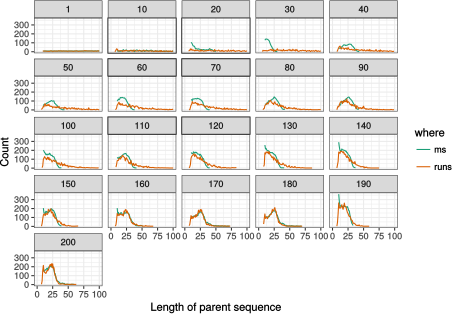
\includegraphics{sea_2018_files/figure-latex/unnamed-chunk-1-1.pdf}

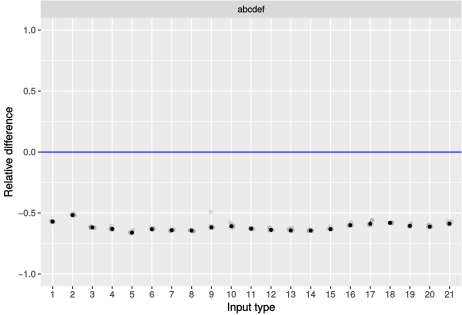
\includegraphics{sea_2018_files/figure-latex/unnamed-chunk-2-1.pdf}
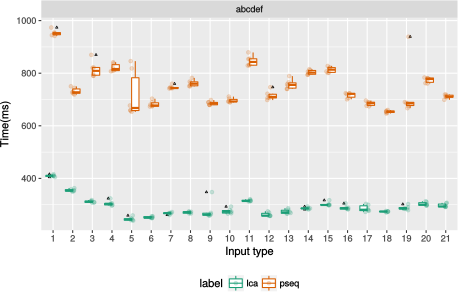
\includegraphics{sea_2018_files/figure-latex/unnamed-chunk-2-2.pdf}

\section{Genome tests}\label{genome-tests}

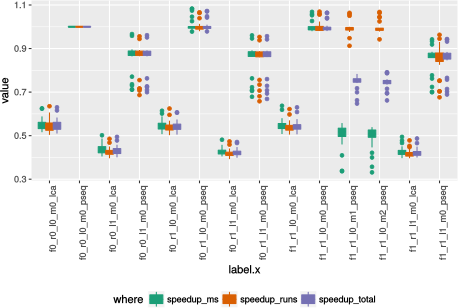
\includegraphics{sea_2018_files/figure-latex/genome-tests-1.pdf}


\end{document}
